\section{Methodology}
\label{Methodology}
The realization of our architecture can be divided in to two distinct stages: First we will leverage existing technologies to establish the framework for our system, in particular connectivity, reachability, and basic services.  
Second, we will build new technologies and applications to provide the key functionality of our decentralized system.

\subsection{Framework}
% Our framework can be divided in to two stages.  
% The first stage leverages existing "`off-the-shelf"' technologies to provide the foundation of our architecture.
% The second stage involves developing new technologies and applications to provide the key functionality of our decentralized system.
% 
%\subsubsection{Foundation of Exisiting Technologies}
The first step in realizing our architecture is establishing connectivity and reachability to our devices.
As discussed in Section~\ref{sec:relconn}, existing work has already addressed, and largely solved, this issue, thus it will not be our focus.
Unfortunately these methods have not been widely deployed, are blocked, or have only been tested in lab settings.
%While there are existing technologies which address this issue, as discussed in Section~\ref{sec:relconn}, these methods have not been widely deployed, are blocked, or have only been tested in lab settings.
%Since this is not our area of focus, we 
To bypass this challenge, we intend to use a VPN server, such as OpenVPN~\cite{feilner2006openvpn}, running on an RECG lab server to allocate static public IPs to our devices.
We hope that this will enable our devices to be publicly accessible, as well as provide a reliable way for them to communicate with each other.
However, if this approach fails, we may have to fall back to other methods such as UIA~\cite{ford2008uia,ford2006persistent}, or limit the scope of our experiments.

The next component in our architecture is device naming and management.
Conventional DNS provides human friendly names as well as domain management, and, in more advanced systems can also provide load-balancing and failover.
In our architecture we will additionally use it help specify our personal "`mini-clusters"' and failover order.
For example, each group member will have their own sub-domain, then further sub-domains will be used to manage that users' devices and cluster.  Figure ~\ref{Fig.Venn} is an example of a possible namespace.
More specifically we intend to use a name such as "`phone.adriana.recg.rice.edu"' or "`laptop.adriana.recg.rice.edu"' to point to Adriana's phone and laptop respectively, then perhaps "`failover1.adriana.recg.rice.edu"' up to "`failoverN.adriana.rice.edu"' to specify the N failover devices in Adriana's cluster.
Similar naming would be used for each persons' cluster.
Notably these names would only be used internally, and would not be seen by the users.
While DNS is a centralized service, thus breaking our decentralized mantra, we use it out of convenience and time considerations; other decentralized naming systems could also be used similarly, such as the one proposed in UIA.

\begin{figure}[h]
	\begin{center}
	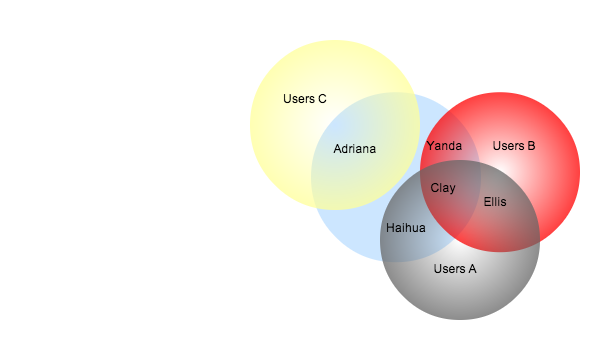
\includegraphics[width=2.5in]{venn.png}
	\caption{Example Namespace.}
	\label{Fig.Venn}
	\end{center}
\end{figure}

The final "`off-the-shelf"' component of our framework is open-source server software, such as postfix, sendmail, apache, etc., which will provide the basis of our communication services.
Combined with the reachability and naming described above, this provides a complete framework for our decentralized framework, which should provide full communication and service, which are even backwards compatible with the existing email and web services.
However, this framework lacks two key features: redundancy and failover.
Additionally, this framework provides some unique opportunities for optimization, which we elaborate on below.
\begin{comment}

%note from Clay:  This is good, but it's probably getting a bit too detailed, especially since a lot of it we either won't be using, or is fairly standard.  Our VPN should take care of all of this since it will assign public static IPs, though DyDNS and UIA may be good to mention as fallbacks.
%Yeah, it's more background stuff.

%The Internet Domain Name Systems (DNS) provides a method for addressing computers based on host or computer names that resolve to specific IP addresses. 
%DNS also allows for directory like services such as Alias or Canonical Names, and services such as Mail Exchange records.   
%Additionally, multiple IP addresses might be configured to correspond to a single host name entry, which helps provide for fault tolerance and load balancing.
%Though the Time-To-Live, or TTL, of a record can be set to zero, numeric IP address changes for a specific DNS record must be updated manually.
%Dynamic Host Configuration Protocol (DHCP) allows for hosts to obtain dynamic IP addresses when they are connected to the network, but this can lead to problems with DNS entries as an IP address might change.
%Dynamic DNS, however, provides a means for automatically updating the DNS record of a host when the host’s IP address changes.
%This is accomplished by using a small piece of software on the host computer that periodically notifies a DNS server of the host’s IP address.
%Such Dynamic DNS providers include DNS Dynamic, Change IP, No-IP, Dyn-DNS, and Zone Edit.
%In UIA, the requestor leases a name entry from a responder for a certain period of time.
%The responder can then notify the requestor when the underlying IP address changes.
%Additionally, the devices in UIA operate in an overlay routing protocol so that changes in IP addresses or Network Address Translation can be resolved into location independent connectivity \cite{ford2008uia,ford2006persistent}.
%Virtual Private Network connections allow a computer to utilize a network as if it were connected directly to the network, even when it is on another network.
%A VPN can provide local IP addresses to the network as well as access to local services.
%Mobile IP is an open standard that can give a mobile device the appearance of having a static IP address even when the device changes to a new network and gets a new physical IP address.  It works by devices having a Home Agent that forwards information to the mobile device through a Foreign Agent when the mobile device is not on the home network.

 DNS
 VPN
 Public IP
 Open source
 
 1 Server with public IPs
 
 2 installing server email...
 
 3. setup DNS 
 
The first stage of this project would be to install (or perhaps port)
open-source server software, e.g. Apache, Jetty, postfix, sendmail, etc., to a
phone.  The next stage would be to ensure reachability from the Internet.  Some
work has already been done here, such as UIA [2]; however, since IPv6 and
MobileIP already address this issue,

it may be best to focus on other challenges
which are more novel.  In the meantime we could use a custom APN (which Rice may
already have), or VPN, to assign a public IP to the phones.  The final research
stage of the project could take one of many directions including ensuring data
redundancy, uptime measurements, distributing loads, power consumption,
encryption, etc.  Perhaps, since this is a networking course, the focus should
be on how to maintain seamless connectivity on node failure in such a system
(beyond simple DNS failover).
\end{comment}
%
%
\subsection{Performance Metrics and Analysis}
Once we have built our decentralized architecture, it is critical to analyze its performance.
We will analyze:
\begin{itemize}
 \item Uptime, Reachability, and Failover
 \item Failure Resistance and Recovery
 \item Load balancing and power efficiency
\end{itemize}

\subsection{Key Issues}
Even when building a decentralized architecture, we are still required to provide reliability by having 100\% availability of the data and fast accessibility. 
In order to achieve the goals of reliability, 100\% availability and fast accessibility, our system must overcome the following.

\textbf{Failover.}  %note from Clay:  actually it is quite the opposite -- there is no signle point of failure in a decentralized system... that is one of the main advantages we are arguing for.
%the issue is just detecting the failure and moving on to the next device in line to accept the request.
% Yes that is the point I was trying to make, let me reword.
In a decentralized architecture, the number of point of failures are increased. 
In a centralized architecture, if a central server fails, it is easily trackable and detectable.
However, in the case of a distributed architecture, the points of failure are multiplied. 
Even though, multiple point of failures is helpful in security purposes, it makes the system more prone to errors because detecting the failure is harder to then activate failover mechanism.
In order to address this issue, our system relies on data replication or redundancy. 
Data will be distributed across multiple nodes, where we will provide a redundancy level that is proportional to the size of the network and load.

Furthermore, we identify there exist varying requirements in failover strategies for different applications. 
In the case of real-time applications, such as chat or VoIP, if the user is unavailable or offline, there is no necessity in activating failover to other people's devices. 
Instead, failover for real-time applications should occur between the devices of the same owner. 
For example, if my phone is unavialble, my calls can failover to any other of my active devices.

In general, by storying multiple copies of the data our system will combat failovers. 
Moreover, our system will consider application base failover possibilities. 
Furthermore, as explained bellow, our system will take into consideration device capabilities for data distribution, thus reducing the possibility of failovers from power outage or other device dependent issues.

\textbf{Diversity in Device Capability.}
Since, data will be store in various types of devices, our system is required to be robust to the different device capabilities. 
A key example of diverse capability is power or battery life. Some devices might be able to have longer up-time than others, thus our system is required to adapt to such differences. 
A possible approach is power adaptation, by analyzing remaining battery life of a device, to then perform decisions of reducing transmission power or even remove such device from the cluster. 
Another example of diverse capability is the storage capability of a device. Some devices might be capable of storing larger amounts of data than others. 
Overall, our system will approach different device capabilities by analyzing each device, building a feedback infrastructure and performing decisions based on each device capability. Through this we ensure data distribution is performed properly in order to achieve our goals.
% 
%Clay: an interesting thing to note here may be the privacy issue.  While the decentralized architecture is more private from a "`big brother"' aspect, it seems that in many other cases it may be a huge problem, as many of the things we want kept private are from our friends/family (whereas we don't necessarily care if google knows).  
% For example, say I have a doctors appointment that I don't want my friends to know about, but my device goes offline, and the email gets sent to their device.  
% Obviously the system doesn't intentionally tell the friend I just received an email from my doctor, but it would be trivial for them to figure it out...  (even if it were encrypted using something like pgp, it wouldn't hide the sender's IP...)  Maybe we can find a way around this?
% 

\textbf{Mode of Connectivity.}
Different modes of connectivity will be supported and tested for different devices.
For instance, a mobile phone could connect to the framework using a Wi-Fi connection direct to local network services.
Alternatively, it could connect using a VPN through a cellular telephone network.
Ideally, the device should make a connection that supports the best overall user experience for the device user as well as the users consuming services provided by the mobile device.  Bluetooth would be another possible connection mode, but is probably beyond the scope of this project.   Laptop devices could connect in a wired or wireless fashion to the framework. Each connectivity method would consume a different set of resources and provide a different level of service.  In our project we would like to not only make the method of connectivity as easy as possible for the end user, but will also measure the performance tradeoffs of connectivity modes.
\begin{comment}
For our project, the mode of connectivity should be wireless combining with wire. 
The desktop computers use wire connecting with the AMAZON EC3, but the rest parts use wireless connecting with each other. 
Bluetooth is an alternative connectivity, but we think it cannot be used very commonly. Not each device will turn on the bluetooth because of the easily consumption of battery. 
In conclusioin, the mode of connectivity based on wireless between different operating system, like mobile system for Andriod and iOS and desktop system for Windows and MAC OS X.
\end{comment}